\section{Results}
\label{sec:results}

% ── Instructions ─────────────────────────────────────────────────────────
% State results quantitatively first, then explain/discuss.
% Every table and figure must be referenced in the text before it appears.
% Use \pm for standard deviation. Avoid qualitative-only claims.
% ─────────────────────────────────────────────────────────────────────────

\subsection{Trajectory Accuracy}

Table~\ref{tab:ate} summarises the Absolute Trajectory Error for baseline
and constrained conditions.
Camera constraints reduce mean ATE from \textbf{?~m $\pm$ ?~m} to
\textbf{?~m $\pm$ ?~m}, a \textbf{?\%} improvement.

\begin{table}[t]
    \centering
    \caption{Absolute Trajectory Error (ATE) across 5 runs ($\downarrow$ better).}
    \label{tab:ate}
    \begin{tabular}{lcc}
        \toprule
        \textbf{Method} & \textbf{Mean ATE (m)} & \textbf{Std (m)} \\
        \midrule
        Vanilla SLAM               & --   & -- \\
        Camera-constrained (ours)  & --   & -- \\
        \bottomrule
    \end{tabular}
\end{table}

\subsection{Map Consistency}

Figure~\ref{fig:map_comparison} shows occupancy maps produced after one full
lap of the ring environment.
The baseline map shows \textasciitilde\textbf{?\%} overlap with ground
truth, while the constrained map achieves \textbf{?\%}.

\begin{figure}[t]
    \centering
    \begin{subfigure}[b]{0.48\linewidth}
        \centering
        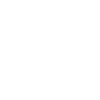
\includegraphics[width=\linewidth]{figures/map_baseline.png}
        \caption{Vanilla SLAM.}
    \end{subfigure}
    \hfill
    \begin{subfigure}[b]{0.48\linewidth}
        \centering
        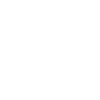
\includegraphics[width=\linewidth]{figures/map_constrained.png}
        \caption{Camera-constrained (ours).}
    \end{subfigure}
    \caption{Occupancy maps after one full lap of the ring world.
             Ground-truth walls overlaid in red.}
    \label{fig:map_comparison}
\end{figure}

\subsection{Camera Marker Error}

The mean Euclidean error between estimated (orange) and ground-truth
(yellow) camera positions is reduced from \textbf{?~m} to
\textbf{?~m}, confirming that the constraint injection correctly anchors
the map frame.

\subsection{Covariance Sensitivity}
\label{sec:cov_sensitivity}

% TODO: sweep sigma values and report ATE table or curve.
Figure~\ref{fig:sigma_sweep} shows ATE as a function of $\sigma_x$ for
fixed $\sigma_\theta = 0.05$.
Over-tightening ($\sigma_x < 0.05\ \si{\metre}$) causes the solver to
over-correct spurious detections, increasing error.
Values in the range $[0.08, 0.15]\ \si{\metre}$ are consistently beneficial.

\begin{figure}[t]
    \centering
    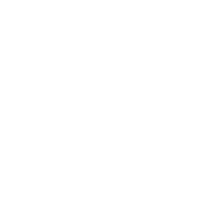
\includegraphics[width=\linewidth]{figures/sigma_sweep.pdf}
    \caption{ATE vs.\ constraint standard deviation $\sigma_x$.
             Shaded region shows $\pm 1$ standard deviation over 5 runs.}
    \label{fig:sigma_sweep}
\end{figure}

\subsection{Discussion}

% ── TODO: fill in after running experiments ───────────────────────────────
The results demonstrate that even a small number of fixed cameras
(one per room) provides sufficient anchoring to suppress drift in a
loop-closing environment.
The primary failure mode is false-positive detections when the robot is
partially occluded; future work can address this with a confidence threshold
on the YOLO detection score before injecting a constraint.
